\begin{frame}
    \frametitle{Formulation of SDE: $DTMC \to CTMC + ME \to SDE$}
    \begin{textblock*}{50mm}(5mm, 10mm)
        To fix ideas, we recall the
        deterministic philosophy to
        formulate ODEs
        \begin{enumerate}[label=(\roman*)]
            \item<2-> 
                We study a process in an small interval of
                time $\Delta t$
            \item<3->
                Describe the resulting information in $\Delta t$
            \item<4->
                Letting $\Delta t \to 0$ gives an ODE
        \end{enumerate}
    \end{textblock*}
% %
     \only<5>{
         \begin{textblock*}{50mm}(70mm, 10mm)
            \begin{exampleblock}{Newton's Cooling Law}
                $
                    T_A(t + \Delta t) - T_A(t) = 
                        \alpha (T_B - T_A(t)) \Delta t
                $
                $   \displaystyle
                    \frac{T_A(t + \Delta t) - T_A(t)}{\Delta t}
                    = \alpha (T_B - T_A(t)) 
                $
                Letting $\Delta t \to 0$
                $$   \displaystyle
                    \frac{dT_A(t)}{dt}
                    = \alpha (T_B - T_A(t))
                $$
            \end{exampleblock}
        \end{textblock*}
        \begin{textblock*}{60mm}(75mm, 47.5mm)
            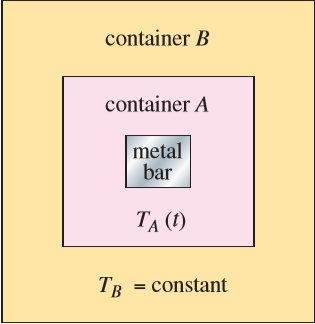
\includegraphics[width=0.7\linewidth]{noise/Images/Assets/newton_cooling_law}
        \end{textblock*}
    }
\end{frame}
% %
\begin{frame}
    \frametitle{Formulation of SDE: $DTMC \to CTMC + ME \to SDE$}
%
        \begin{textblock*}{60mm}(5mm, 15mm)
            A stochastic analogy.
            \begin{enumerate}[label=(\roman*)]
                \item<2->
                    Formulate a discrete stochastic
                    model for the dynamical system
                    understudy, which describe changes
                    in a small time interva $\Delta t$
                \item<3->
                    Compute the expected value and
                    covariance for the difference in a short
                    time $\Delta t$
                \item<4->
                    Letting $\Delta t \to 0$, 
                    he above information
                    leads to the CTMC
                \item<5->
                    Thus, we infer the SDE from the
                    similarities in the forward-backward-Kolmogorov equation 
                    between the
                    discrete and Continuous Markov
                    Chain
            \end{enumerate}
        \end{textblock*}
\end{frame}
% %
\begin{frame}% frame 00
    \frametitle{Example: Formulation of a stochastic SIS model}
    \begin{textblock*}{50mm}(5mm, 10mm)
    Consider the deterministic SI model:
        \begin{align*}
            \frac{dS}{dt} &= -\frac{\beta}{N} S I + (b +\gamma) I
                \\
            \frac{dI}{dt} &= \frac{\beta}{N} S I - (b +\gamma) I
                \\
            N &= S(t)+ I(t)
        \end{align*}
        Where $N$ is constant and  $S(t) = N - I(t)$.
    \end{textblock*}
    \only<2->{
        \begin{textblock*}{50 mm}(60mm, 10mm)
            \begin{empheq}[box=\shadowbox]{align*}
                \mathcal{R}_0 &= 
                    \frac{\beta}{b + \gamma}
                    \\
                \mathcal{R}_0 & \leq 1
                \\
                & \Rightarrow
                    \lim_{t \to \infty} (S(t),N(t)) = (N, 0)
                \\
                \mathcal{R}_0 & > 1
                \\
                & \Rightarrow
                    \lim_{t \to \infty} (S(t),N(t)) = (S^*, I^*)
            \end{empheq}
        \end{textblock*}
    }
\end{frame}
% %
% %
\begin{frame}{Example: Formulation of a stochastic SIS model}
    \begin{textblock*}{55mm}(5mm, 10mm)
        Consider the process $\{\mathcal{I}_t\}_{t=0} ^ \infty$ with 
        time discrete and space of states $\{0,1,\cdots, N \}$.
        \begin{enumerate}[label=(H-(\arabic*)]
            \item <2->
                \begin{align*}
                    p_i(t) &:= \probX{\mathcal{I}(t) = i}
                    \\
                    i &= 0,1,2\dots, N
                    \\
                    t &= 0, \Delta t, 2 \Delta t, \cdots,
                \end{align*}
            \item <3->
                Markov property
                $$
                    \probCX{I_{t + \Delta t}}{  I_0, I_{\Delta t}, \cdots, I_t}
                    =\probCX{I_{t + \Delta t} }{I_t}
                $$
            \item <4->
                The unique transitions with positive 
                probability
                \begin{align*}
                    & p_{ji}(t + \Delta t)
                    = 
                    \probCX{I_{t + \Delta t} = j}{I_t = i}
                    \\
                    &\text{are}
                    \\
                    & i \to i+1, \ i \to i-1,  \ i \to i
                \end{align*}
        \end{enumerate}
    \end{textblock*}
    \only<5->{
        \begin{textblock*}{50mm}(55mm, 10mm)
            \begin{equation*}
                p_{ji}(\Delta t):=
                    \begin{cases}
                        \frac{\beta i (N - i)}{N} \Delta t, 
                            & j = i + 1
                        \\
                        (b + \gamma) i \Delta t, 
                            & j = i - 1
                        \\
                        1 - 
                        \left[
                            \frac{\beta i (N - i)}{N} +
                            (b + \gamma) i
                        \right]
                        \Delta t, 
                            & j=i,
                        \\
                        0 & \text{otherwise}
                \end{cases}
            \end{equation*}
            where $\Delta t$ is sufficiently small s.t.
            $$
                \max_{i \in \{ 1, \dots, N \}}
                \{
                    [b(i) + d(i)] \Delta t
                \}
                \leq 1
            $$
        \end{textblock*}
    }
    \only<6>{
        \begin{textblock*}{50mm}(65mm, 60mm)
            \begin{center}
                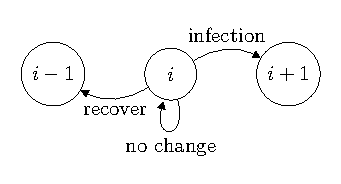
\includegraphics[width=\linewidth]{noise/Images/Assets/chain.pdf}
            \end{center}
        \end{textblock*} 
     }
\end{frame}
%%%%%%%%%%%%%%%%%%%%%%%%%%%%%%%%%%%%%%%%%%%%%%%%%%%%%%%%%%%%%%%%%%%%%%%%%%%%%%%%
\begin{frame}{Example: Formulation of a stochastic SIS model}
    \only<2->{
    \begin{textblock*}{55mm}(5mm, 10mm)
        Letting
        \begin{align*}
            b(i) &:= \frac{\beta i (N - i)}{N} \Delta t
            \\
            d(i) &:= (b + \gamma) i \Delta t
        \end{align*}
    \end{textblock*}
    }
    \only<3->{
        \begin{textblock*}{90mm}(45mm, 8mm)
            \begin{empheq}[box={\Garybox[FKE]}]{align*}
                p_i(t + \Delta t) &=
                    p_{i-1}(t) b(i - 1) \Delta t 
                    \\
                    & + p_{i+1}(t) d(i + 1) \Delta t
                    \\
                    & + p_i(t) (1 -[b(i) + d(i)] \Delta t)
            \end{empheq}
        \end{textblock*}
    }
    \only<4->{
    \begin{textblock*}{140mm}(-3mm, 35mm)
        \hspace{5em} Thus $P(\Delta t) = $
        \begin{equation*}
            \begin{pmatrix}
            1   & d(1) \Delta t & 0 & \cdots    & 0 & 0
            \\
            0   & 1 - (b+d)(1) \Delta t & d(2)  \Delta t   & \cdots    & 0   & 
            0 
            \\
            0   & b(1) \Delta t  & 1 - (b+d)(2) \Delta t   & \cdots    & 0 & 0
            \\
            0 & 0 & b(2) \Delta t & \cdots    & 0 & 0
            \\
            \vdots & \vdots & \vdots & \ddots & \vdots & \vdots
            \\
            0 & 0 & 0 & \cdots & d (N - 1) \Delta t  & 0
            \\
            0 & 0 & 0 & \cdots & 1- (b+d) (N - 1) \Delta t  & d(N) \Delta t
            \\
            0 & 0 & 0 & \cdots & d (N - 1) \Delta t  &  1 - d(N) \Delta t 
            \end{pmatrix}
        \end{equation*}
        \begin{textblock*}{100mm}(10mm, 80mm)
            $$
                p(t + \Delta t) = P(\Delta t) p(t) = P^{n+1}(\Delta t) p(0), 
                \qquad t =n \Delta t
            $$
        \end{textblock*}
    \end{textblock*}
    }
\end{frame}
% %
% %
\begin{frame}{Expected Value of the SIS-DTMC}
    \begin{textblock*}{80mm}(15mm,6mm)
        \begin{align*}
            \only<2->{
                \E(I_{t + \Delta t}) 
                &=  
                    \sum_{i = 0} ^ N
                        i p_i(t + \Delta t)
            }
            \\
            \only<3->{
                &=
                        \sum_{i = 0} ^ N
                            i p_{i - 1} (t) b(i - 1) \Delta t
                    + \sum_{i = 0} ^ {N-1}
                            i p_{i + 1} (t) d(i + 1) \Delta t
                \\       
                    &+ 
                        \sum_{i=0}^N i p_i(t) \Delta t
                        - \sum_{i=0}^N i p_i(t) b(i) \Delta t
                        - \sum_{i=0}^N i p_i(t) d(i) \Delta t
            }
            \\
            \only<4>{
                \E(I_{t+ \Delta t}) 
                    &= 
                    \E(I_t) 
                        + \sum_{i = 1} ^ N
                            p_{i-1} (t)
                            \frac{\beta (i-1)(N - [i -1])}{N} \Delta t
                \\
                        &-
                            \sum_{i = 0} ^ {N - 1}
                            p_{i + 1} (t) (b + \gamma) (i+1) \Delta t
                \\
                    &=
                    \E(I_t) + [\beta - (b + \gamma )] \Delta t \E(I_t)
                    -\frac{\beta}{N} \Delta t 
                    \underbrace{\E(I_t ^ 2)}_{\geq \E ^2(I_t)}
            }
        \end{align*}
    \end{textblock*}
%
\end{frame}
% %%%%%%%%%%%%%%%%%%%%%%%%%%%%%%%%%%%%%%%%%%%%%%%%%%%%%%%%%%%%%%%%%%%%%%%%%%%%%%%%
\begin{frame}{Expected Value of the SIS-DTMC}
    \begin{textblock*}{60mm}(20mm, 25mm)
       \begin{equation*}
            \frac{\E(I_{t + \Delta t}) - \E(I_t)}{\Delta t}
                \leq
                    [\beta  - (b + \gamma)] \E (I_t)
                    - \frac{\beta}{N} \E^2 (I_t)
        \end{equation*}
        %
        \only<2->{
            \begin{align*}
                \frac{d \E(I_{t})}{dt}
                    & \leq
                        [\beta  - (b + \gamma)] \E (I_t)
                        - \frac{\beta}{N} \E ^ 2 (I_t)
                \\
                    & = \frac{\beta}{N} [N - \E(I_t)] \E (I_t)
                        - (b + \gamma) \E (I_t)
            \end{align*}
        }
        \only<3->{
            \begin{empheq}[box=\shadowbox]{equation*}
                \frac{d \E(I_{t})}{dt}
                \leq
                \frac{\beta}{N} \E(S_t) \E (I_t)
                    - (b + \gamma) \E (I_t)
            \end{empheq}
        }
    \end{textblock*}
\end{frame}
%%%%%%%%%%%%%%%%%%%%%%%%%%%%%%%%%%%%%%%%%%%%%%%%%%%%%%%%%%%%%%%%%%%%%%%%%%%%%%%%
\begin{frame}{Example: Formulation of a stochastic SIS model}
    \begin{textblock*}{55mm}(5mm, 10mm)
        \begin{empheq}[box=\shadowbox]{align*}
            N &= 100, \ \Delta t = 0.01, \ \beta = 1, 
            \\
            b &= 0.25 \ \gamma = 0.25 
        \end{empheq}
    \end{textblock*}
%
    \begin{textblock*}{100mm}(5mm, 20mm)
        \begin{center}
            \includegraphics[width=\linewidth]{%
                noise/Images/Assets/random_walk_SIS%
            }
        \end{center}
    \end{textblock*}
%
    \begin{textblock*}{20mm}(105mm, 20mm)
        \begin{empheq}[box=\fbox]{align*}
            \mathcal{R}_0 &= 2,  
             \\
            \bar{I} &= 50
        \end{empheq}
    \end{textblock*}
\end{frame}
% %